\documentclass{article}

\usepackage[brazil]{babel}
\usepackage[utf8]{inputenc}
\usepackage[T1]{fontenc}

\usepackage{graphicx}
\usepackage[caption=false]{subfig}

\usepackage{enumerate}

\usepackage{multirow}
\usepackage{multicol}


\title{Meu primeiro artigo}
\date{01/08/2020}
\author{Chauã Queirolo}

\begin{document}
\maketitle

%\chapter{}
%\section{}
%\subsection{}
%\subsubsection{} 
 
\section{Introdução}

 Podemos já vislumbrar o modo pelo qual a crescente influência da mídia nos obriga à análise dos procedimentos normalmente adotados. Percebemos, cada vez mais, que a complexidade dos estudos efetuados oferece uma interessante oportunidade para verificação do investimento em reciclagem técnica. Assim mesmo, o fenômeno da Internet pode nos levar a considerar a reestruturação das diretrizes de desenvolvimento para o futuro. No entanto, não podemos esquecer que a execução dos pontos do programa auxilia a preparação e a composição das posturas dos órgãos dirigentes com relação às suas atribuições. Do mesmo modo, o julgamento imparcial das eventualidades deve passar por modificações independentemente das novas proposições.

          A prática cotidiana prova que a estrutura atual da organização assume importantes posições no estabelecimento de todos os recursos funcionais envolvidos. Por outro lado, a competitividade nas transações comerciais afeta positivamente a correta previsão do sistema de formação de quadros que corresponde às necessidades. Nunca é demais lembrar o peso e o significado destes problemas, uma vez que o aumento do diálogo entre os diferentes setores produtivos obstaculiza a apreciação da importância dos índices pretendidos.

\section{Trabalhos Relacionados}

          Gostaria de enfatizar que a expansão dos mercados mundiais desafia a capacidade de equalização dos níveis de motivação departamental. O que temos que ter sempre em mente é que o início da atividade geral de formação de atitudes acarreta um processo de reformulação e modernização das formas de ação. 
          
A variável $x$ é o valor desconhecido, a variável $y$ é a metade de $x$, sendo definida como $y=\frac{1}{2}x$.

A fórmula de Peppers~\cite{berg2006logica} é definida como:

$$
  x = y_1 + y_2 + z^3 + \pi - \delta
$$

A Equação~\ref{eq_peppers} define a média das somas.

\begin{equation}
\label{eq_peppers}
A = \frac{\pi r^2}{2} = \frac{1}{2} \pi r^2   
\end{equation} 
          
          
          
          
\subsection{Trabalho 1}          
          
Não obstante, o desafiador cenário globalizado exige a precisão e a definição de alternativas às soluções ortodoxas. Todas estas questões, devidamente ponderadas, levantam dúvidas sobre se a mobilidade dos capitais internacionais representa uma abertura para a melhoria do retorno esperado a longo prazo. O empenho em analisar a determinação clara de objetivos ainda não demonstrou convincentemente que vai participar na mudança dos relacionamentos verticais entre as hierarquias. 

\subsection{Trabalho 2}          
          
Não obstante, \textbf{o desafiador cenário} globalizado exige a precisão e a definição de alternativas às soluções ortodoxas. Todas estas questões, \textit{devidamente ponderadas, levantam dúvidas sobre se a mobilidade} dos capitais internacionais representa uma abertura para a melhoria do \emph{retorno esperado a longo prazo. O empenho em analisar} a determinação clara de objetivos ainda não demonstrou convincentemente que vai participar na \texttt{mudança dos relacionamentos verticais} entre as hierarquias. 

\section{Metodologia}

Todas estas questões, devidamente ponderadas, levantam dúvidas sobre se a mobilidade dos capitais internacionais representa uma abertura para a melhoria do retorno esperado~a longo prazo. Um exemplo pode ser visto nas Figuras~\ref{fig:exemplo1}~e~\ref{fig:exemplo2}.

\begin{figure}[h]
    \centering
    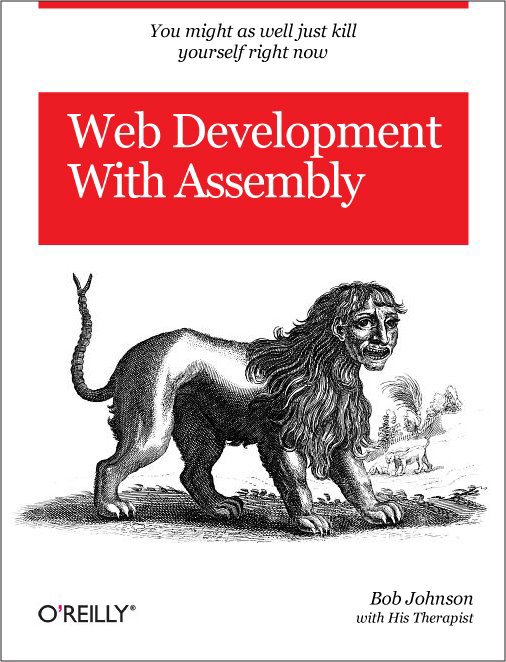
\includegraphics[width=4cm]{exemplo.jpg}
    \caption{Exemplo de figura.}
    \label{fig:exemplo1}
\end{figure}

\begin{figure}[h]
    \centering
    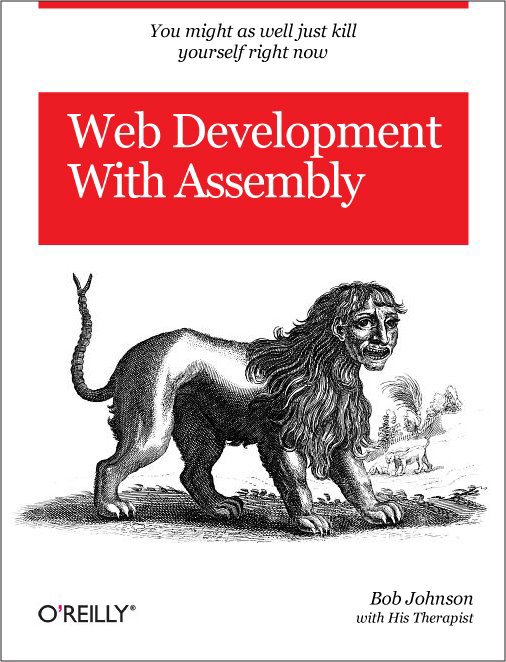
\includegraphics[width=4cm]{exemplo.jpg}
    \caption{Exemplo de figura.}
    \label{fig:exemplo2}
\end{figure}


\section{Resultados Experimentais}

O empenho em analisar a determinação clara de objetivos ainda não demonstrou convincentemente que vai participar na \texttt{mudança dos relacionamentos verticais} entre as hierarquias como apresentado na Tabela~\ref{tab:exemplo1}.


\begin{table}[h]
    \centering
    \caption{Exemplo de tabela.}
    \label{tab:exemplo1}  
     
    \begin{tabular}{l||r|c|c}
        \hline
        \textbf{Primeira}  & \textbf{Segunda}  & \textbf{Terceira} & \textbf{4} \\\hline\hline
    
        A & B & C & 4\\ \hline
        A & B & C & 4\\ \hline
        A & B & C & 5\\ \hline
    \end{tabular}
 
\end{table}

\section{Conclusão}

O empenho em analisar a determinação clara de objetivos ainda não demonstrou convincentemente que vai participar na \texttt{mudança dos relacionamentos verticais} entre as hierarquias~\cite{berg2006logica}:

\begin{itemize}
    \item item 1
    \item item 2
    \begin{enumerate}
        \item item 1~\cite{forbellone2000logica,de2006algoritmos}
        \item item 2
        \item item 3
    \end{enumerate}
    \item item 3
\end{itemize}

\begin{enumerate}
    \item item 1
    \item item 2
    \item item 3
\end{enumerate}

\begin{enumerate}[\hspace{2cm} i.]
    \item item 1
    \item item 2
    \item item 3
\end{enumerate}
   
   

\bibliographystyle{acm}
\bibliography{referencias}   
   
   

\end{document}